\section{Семинар 2}

\subsection{Издержки}

\textbf{Издержки} (затраты) делятся на постоянные и переменные. Признак разделения: какова динамика затрат в соответствии с изменением объемов выпускаемой продукции.

\textbf{Постоянные затраты} -- это затраты, величина которых в короткосрочном периоде не меняется при изменении объемов выпускаемой продукции.

Например:

\begin{itemize}
    \item затраты на аренду и оборудование;
    \item амортизация оборудования;
    \item проценты по кредитам;
    \item заработная плана управленческому и вспомогательному персоналу.
\end{itemize}

\textbf{Переменные затраты} -- это затраты, величина которых меняется при изменении объемов выпускаемой продукции.

Например:

\begin{itemize}
    \item затраты на покупку материала, сырья;
    \item заработная плата рабочим;
    \item топливо или энергияю
\end{itemize}

\textbf{Внешние издержки} -- это платежи фирмы за приобретамые ресурсы (труд, земля, капитал, информация).

\textbf{Внутренние издержки} -- это доходы, которые могли бы быть получены владельцем фирмы при ином варианте использования своих собственных ресурсов и возможностей.

\textbf{Объем продаж} -- это доход от продажи продукции.

\textbf{Себестоимость продукции} показывает, во сколько предприятию обошлось приобритение или изгтовление товаров.

\subsection{Формирование розничной цены}

\begin{figure}[H]
    \centering
    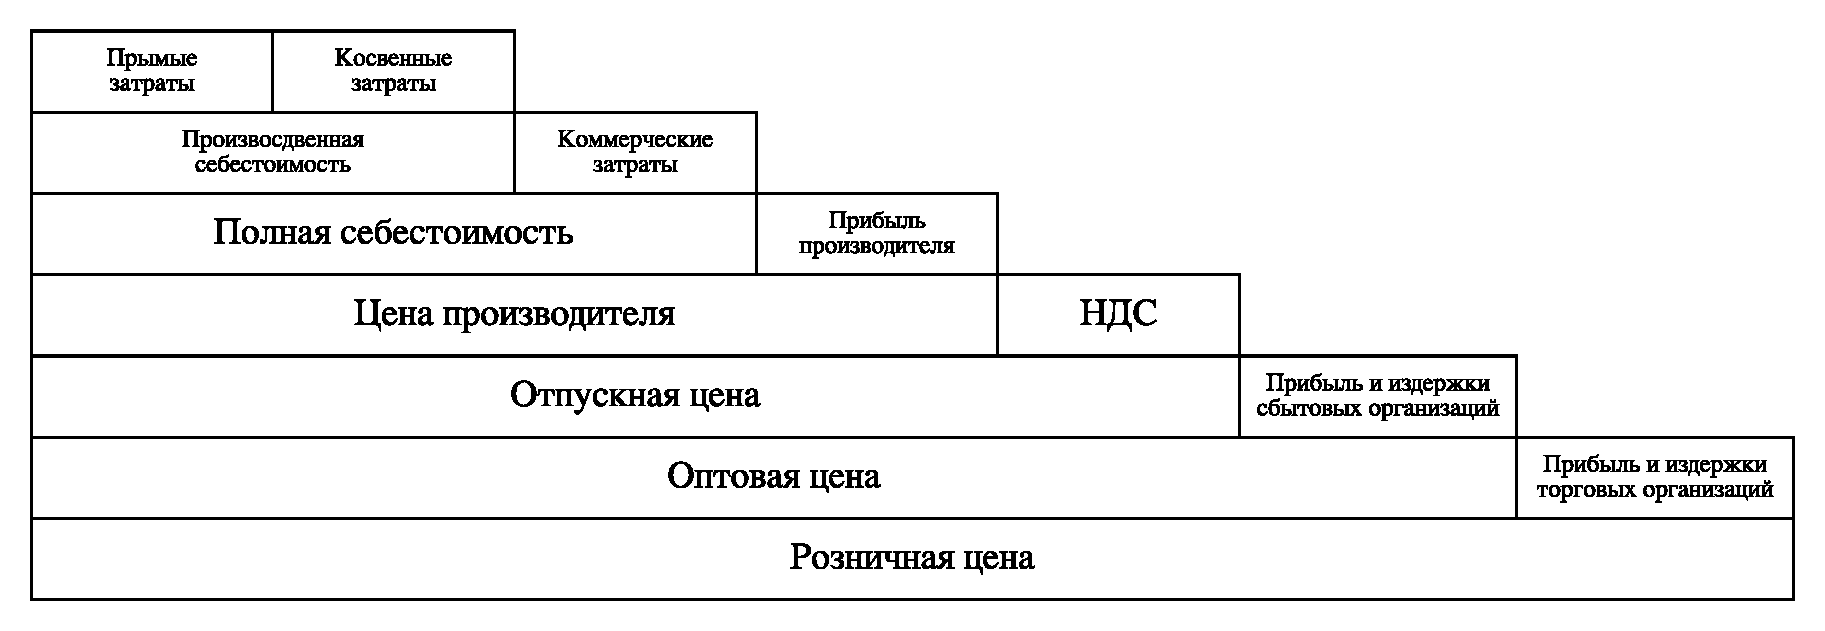
\includegraphics[scale=0.5]{img/cost.pdf}
\end{figure}

\subsection{Взаимосвязь показателей прибыли}

\begin{figure}[H]
    \centering
    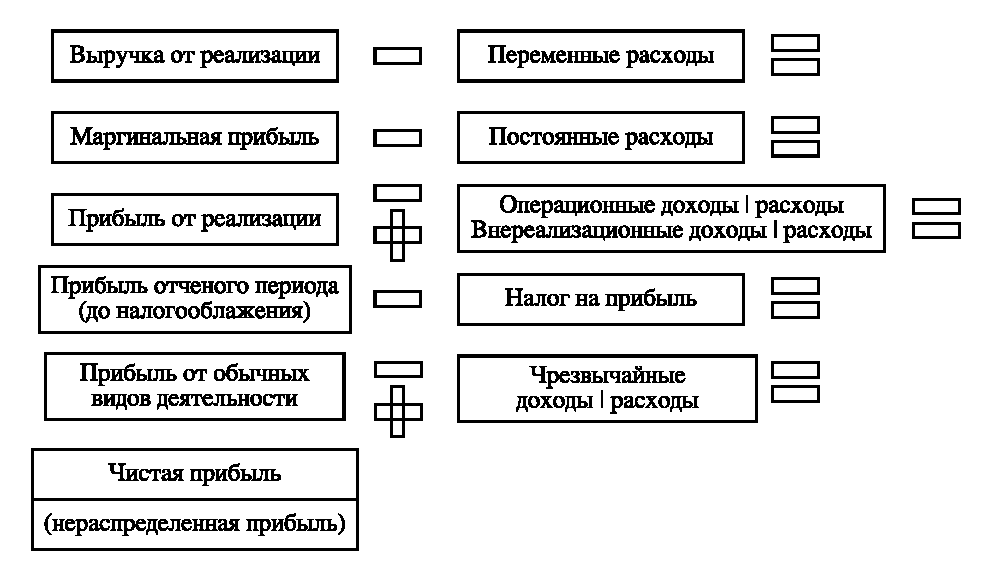
\includegraphics[scale=0.8]{img/relationship.pdf}
\end{figure}

\textbf{Операционные доходы | расходы} -- связаны с предоставлением за плату во временное пользование активов предприятия, прав возникающих из патентов на изобретения, промышленные образцы и других видов интеллектуальной собвственности.Проценты, выплачиваемые предприятием за предоставление ему в пользование денежных средств (кредиты, займы). Продажа, выбытие, списание основных средств или иных активов.

\textbf{Внереализационные доходы | расходы} -- это штрафы, пени, неустойки за нарушение условия договоров. Активы, полученные безвозмездно, в том числе договоры дарения, поступления в возмещение причинных оргинизации убытков (прибыль прошлых лет, сумма до оценки активов).

\textbf{Чрезвычайные доходы | расходы} -- это поступления, возникающие как последствия чрезвычайных обстоятельств в хозяйственной деятельности (стихийные бедствия, пожары, аварии, национализация, страховые возмещения).


\begin{equation*}
    \underbrace{\text{ВП}}_\text{валовая прибыль} = \underbrace{V_\text{п}}_\text{объем продаж} - \underbrace{S}_\text{себестоимость}
\end{equation*}

\begin{equation*}
    \underbrace{\text{ЧП}}_\text{чистая прибыль} = \underbrace{\text{ВП}}_\text{валовая прибыль} - \underbrace{\text{Р}}_\text{расходы}
\end{equation*}

\subsection{Задача 1}

ЧП = 150000

$P$ = 45000

$S$ = 100000

$V_\text{п}$ = ?

\begin{equation*}
    V_\text{п} = 150000 + 45000 + 100000 = 295000
\end{equation*}

\textbf{Рентабельность предприятия} -- это отношение фактической прибыли к объему продаж.

\begin{equation*}
    \underbrace{\text{ЧМ}}_\text{чистая маржа} = \frac{\text{ЧП}}{V_\text{п}} \cdot 100 \%
\end{equation*}

\begin{equation*}
    \underbrace{\text{ВМ}}_\text{валовая маржа} = \frac{\text{ВП}}{V_\text{п}} \cdot 100 \%
\end{equation*}

\begin{equation*}
    \text{Наценка} = \frac{\text{ВП}}{S} \cdot 100 \%
\end{equation*}

\subsection{Задача 3}

$V_\text{п}$ = 200000

$S$ = 90000

$P$ = 30000

ЧМ = ?, ВМ = ?

\begin{equation*}
    \text{ЧМ} = \frac{200000 - 90000 - 30000}{200000} \cdot 100 \% = 40 \%
\end{equation*}

\begin{equation*}
    \text{ВМ} = \frac{200000 - 90000}{200000} = 55 \%
\end{equation*}

\begin{equation*}
    \text{Наценка} = \frac{200000 - 90000}{90000} \cdot 100 \% = 122.22 \%
\end{equation*}
